\chapter{Application}

This chapter outlines the application development process, from design to testing and validation, focusing on the steps taken to ensure functionality, quality, and alignment with the project goals. The development process involved defining the core features of the application, selecting appropriate models, designing interaction protocols, and structuring the system architecture. By following industry best practices, the application was built to facilitate efficient data preprocessing and code generation. The effectiveness of the application was assessed using performance metrics to ensure that it met the required standards. The key steps in the design, development, and testing phases are outlined below.

\section{Design Phase} 
To ensure high quality and robustness, industry-standard best practices were followed during the design phase. This phase is crucial as it defines the application's requirements, architecture, and core functionalities, ensuring they align with user needs and quality standards. The design approach involved the following key steps:

\begin{enumerate} 
    \item Research and selection of the most suitable Large Language Model (LLM) for the project, based on specific performance requirements and available computational resources. 
    \item Comprehensive definition of the application's core functionalities and requirements, ensuring alignment with the project's objectives. 
    \item Identification of key dataset information and metrics essential for accurate code generation (e.g., data distributions, missing value patterns). 
    \item Design of interaction protocols with the LLM, including prompt engineering and fine-tuning methodologies where feasible. 
    \item Detailed architectural design of the application, defining system components and their interactions. 
    \item Specification of evaluation metrics to assess the application's performance and quality. 
    \item Formulation of test strategies to validate the application's functionality and robustness. 
\end{enumerate}

\subsection{Model Selection}
An in-depth review of available LLMs was conducted, with a focus on open-source models to ensure flexibility and ease of customization. Among the models evaluated, Qwen2.5 was selected due to its robust performance metrics within the open-source domain, offering a balanced trade-off between computational efficiency and processing capability at 1.5 billion parameters. Qwen2.5's accessibility via the Hugging Face repository made it a reliable choice for integration, and its architecture was deemed capable of handling preprocessing code generation with the required level of detail and accuracy.

Additionally, the LLama model was evaluated as a potential alternative. LLama has been recognized for its strong performance in a range of natural language processing tasks, offering scalability and versatility. The evaluation process compared both models based on various factors, including model size, computational efficiency, and their ability to generate accurate and relevant preprocessing code. While both models presented distinct advantages, the decision on which to use was made after considering the specific requirements of the project, with the aim of achieving optimal performance for code generation tasks.

\subsection{Functionality and Requirements Definition}
Once the model was selected, the essential features of the application were defined. The goal was to create an application that simplifies data preprocessing for users with varying levels of expertise, including those with minimal experience in data handling. The application was designed to guide users through the process of generating a preprocessed dataset that meets machine learning standards, derived from a raw input dataset. A user-friendly interface was prioritized and implemented using a client-server architecture to separate front-end user interactions from back-end processing tasks.
The core functionalities of the application include:
\begin{itemize}
    \item Automated code generation for data preprocessing tasks, tailored to the input dataset's characteristics.
    \item User-friendly interface for uploading datasets and viewing generated code snippets.
    \item Integration with the Qwen2.5 model for efficient data profiling and preprocessing code generation.
    \item Support for diverse data types and preprocessing requirements, ensuring broad applicability across datasets.
\end{itemize}

\subsection{Data Analysis Requirements}
To optimize code generation, critical dataset metrics were specified for extraction to inform the LLM's response. Key metrics include mean, standard deviation, null value counts, and unique value counts for each dataset column. These metrics provide a comprehensive data profile, enabling the LLM to generate precise preprocessing code tailored to the characteristics of each input dataset. This approach was initially tested on a small dataset using a subset of these metrics to validate and refine the logic, and was later adapted to accommodate larger datasets with varying complexities.

\subsection{Interaction Protocols with the LLM}
The initial approach involved direct interaction with the LLM, without specific adaptations to tailor it to the data engineering tasks required for the project. This baseline interaction provided insights into the model's natural performance and limitations when tasked with generating preprocessing code based on general dataset descriptions.

Subsequently, fine-tuning was considered as a method to enhance the model's alignment with the task by training it on domain-specific examples. While fine-tuning was anticipated to improve the model's accuracy and relevance, limited computational resources on the experimental machine made this approach unfeasible.

As an alternative, a lightweight solution was implemented through prompt engineering. By carefully crafting input prompts, the model's responses were guided to better address the data engineering requirements, simulating the role of a data engineer. Although this approach was less efficient than fine-tuning, it provided an improved level of adaptation to the problem, enhancing the model's ability to generate accurate and useful preprocessing code.

Given the vast and complex nature of the problem domain, a multi-layered conversational approach was also adopted. The problem was decomposed into multiple sequential stages, using distinct prompts for each phase to generate intermediate results. These intermediate outputs were then fed into subsequent interactions, allowing the model to progressively build towards a comprehensive solution. This step-by-step approach facilitated a structured exploration of the problem and yielded more precise final results.

\subsection{Two-Tier Architecture}
A two-tier architecture was adopted to structure and streamline the workflow for data preprocessing and code generation, enhancing code quality and facilitating integration into various projects. This architecture comprises the following stages:

\begin{enumerate}
    \item \textbf{Logic Development:} In the initial tier, the Qwen2.5 model was interacted with using essential dataset metrics—such as mean, standard deviation, null counts, and unique values—to outline a logical structure for data preprocessing. This phase identified primary preprocessing tasks, including data cleaning, scaling, encoding, and missing value handling. By establishing a robust logical framework, this stage ensured that the generated code addressed all necessary preprocessing steps effectively.
    
    \item \textbf{Code Generation:} In the second tier, the preliminary logic was refined into optimized, executable Python code. The generated code was designed to be efficient, readable, and adaptable, supporting modular updates and customization as project requirements evolved. This phase focused on translating the preprocessing logic into high-quality, production-ready code, capable of being seamlessly integrated into various workflows.
\end{enumerate}

This two-tiered approach produced code that was practical, reliable, and versatile, capable of handling diverse preprocessing scenarios with minimal user input. By dividing the process into distinct stages, the architecture supported modular updates and feature additions, providing a scalable solution for both small-scale analyses and complex, data-intensive applications. Figure \ref{fig:architecture} illustrates the architectural layout of this approach, highlighting each stage's role in generating a high-quality preprocessing pipeline.

\begin{figure}[H]
    \centering
    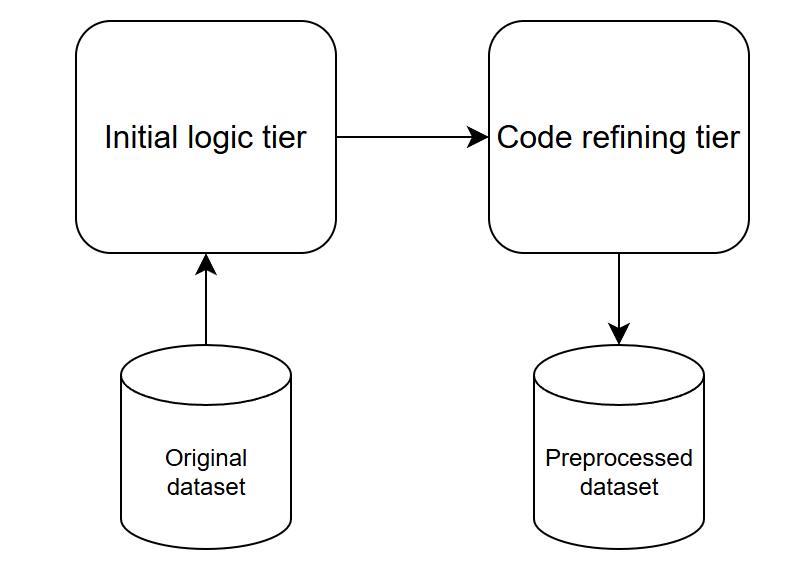
\includegraphics[width=0.5\textwidth]{media/image.png}
    \caption{Architecture of the Proposed Two-Tier Approach}\label{fig:architecture}
\end{figure}

By separating the preprocessing and code generation workflow into these two distinct phases, efficiency was maximized, potential error rates were reduced, and the output met the project's high standards of quality and functionality. This design provides a robust, scalable solution for automated data preparation, accommodating applications ranging from exploratory analyses to large-scale production environments where consistency and quality are essential.

\subsection{Evaluation Metrics}
To rigorously assess the effectiveness of the application, performance metrics focused on code accuracy, usability, and consistency were established. These include:
\begin{itemize}
    \item \textbf{Code Accuracy:} Measuring how accurately the generated code addresses the preprocessing requirements.
    \item \textbf{Usability:} Evaluating the code's readiness for direct use without extensive modifications.
    \item \textbf{Consistency:} Ensuring the application consistently produces reliable results across diverse datasets and preprocessing tasks.
\end{itemize}

\subsection{Testing and Validation}
To validate the application's functionality, tests were conducted using two representative datasets, covering a range of data types and preprocessing needs. These tests assessed the model's ability to generate correct and efficient code in line with the defined requirements, ensuring that the application met both performance and quality benchmarks. The testing phase verified that the application's output aligned with the quality objectives, confirming its readiness for deployment and real-world use.

\section{Mockup of the Application Interface}

\begin{figure}[H]
    \centering
    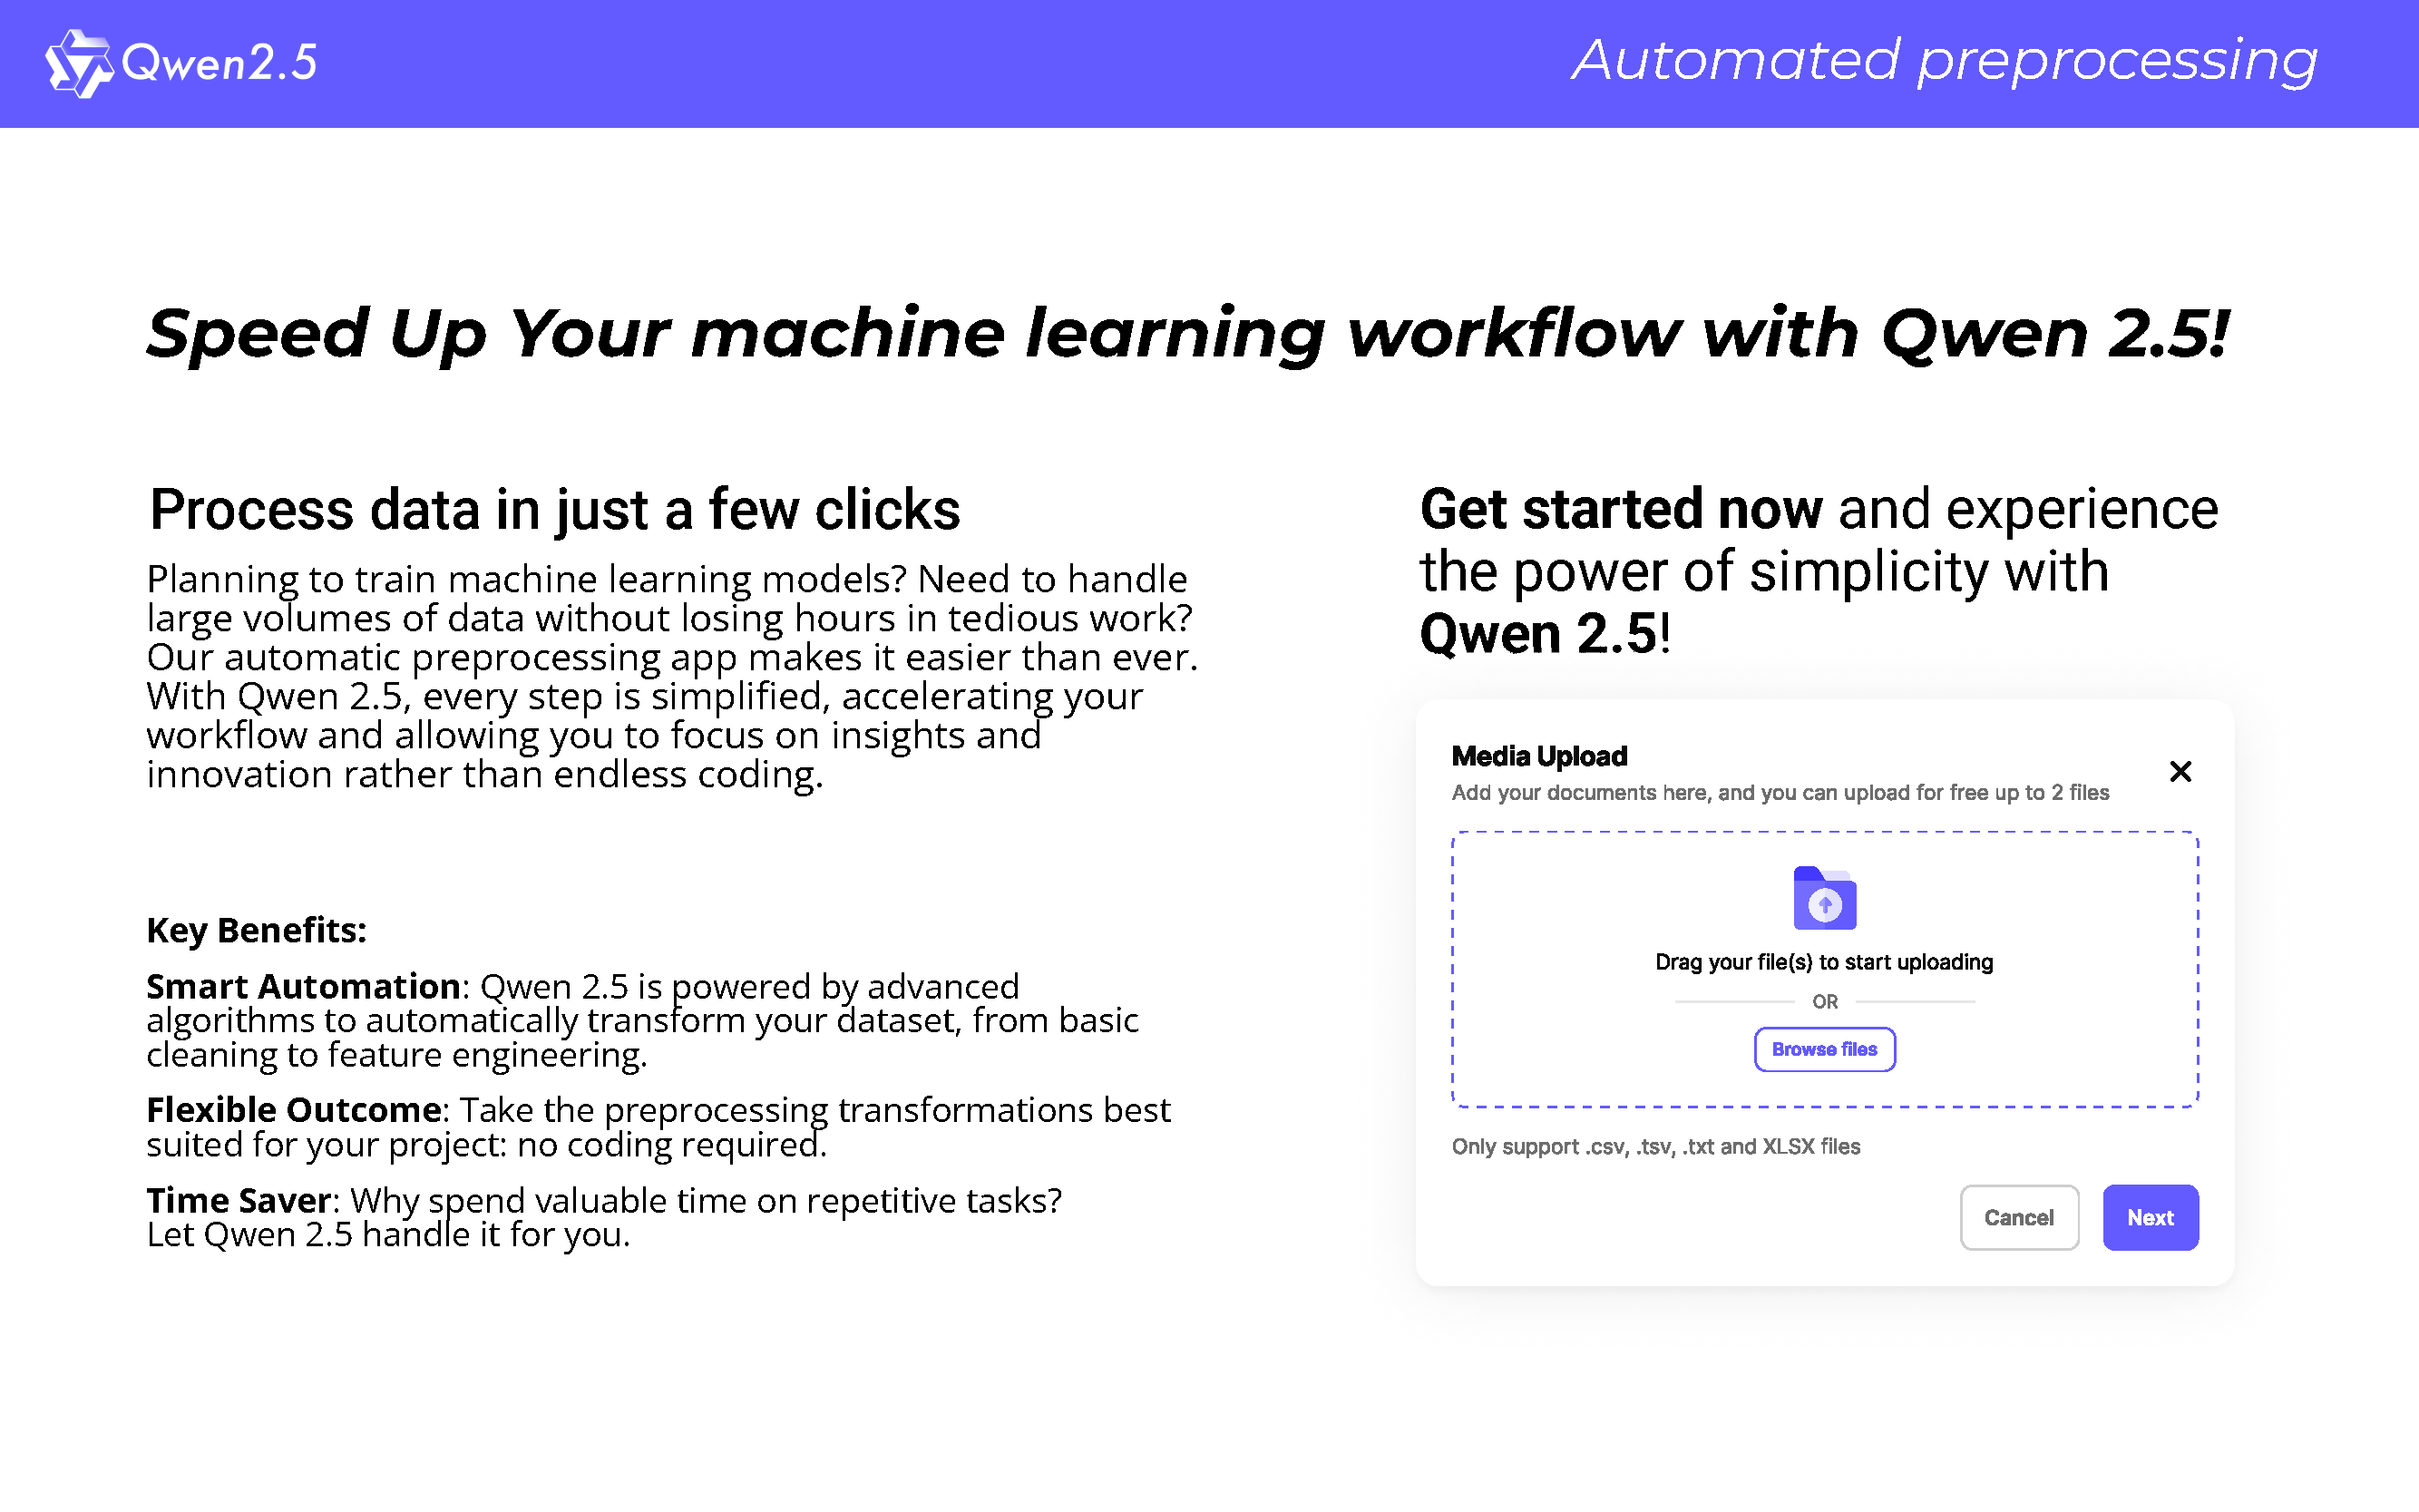
\includegraphics[width=1\textwidth]{media/App_prototipo_1.pdf}
    \caption{Main Page}\label{fig:app_mockup_1}
\end{figure}

\begin{figure}[H]
    \centering
    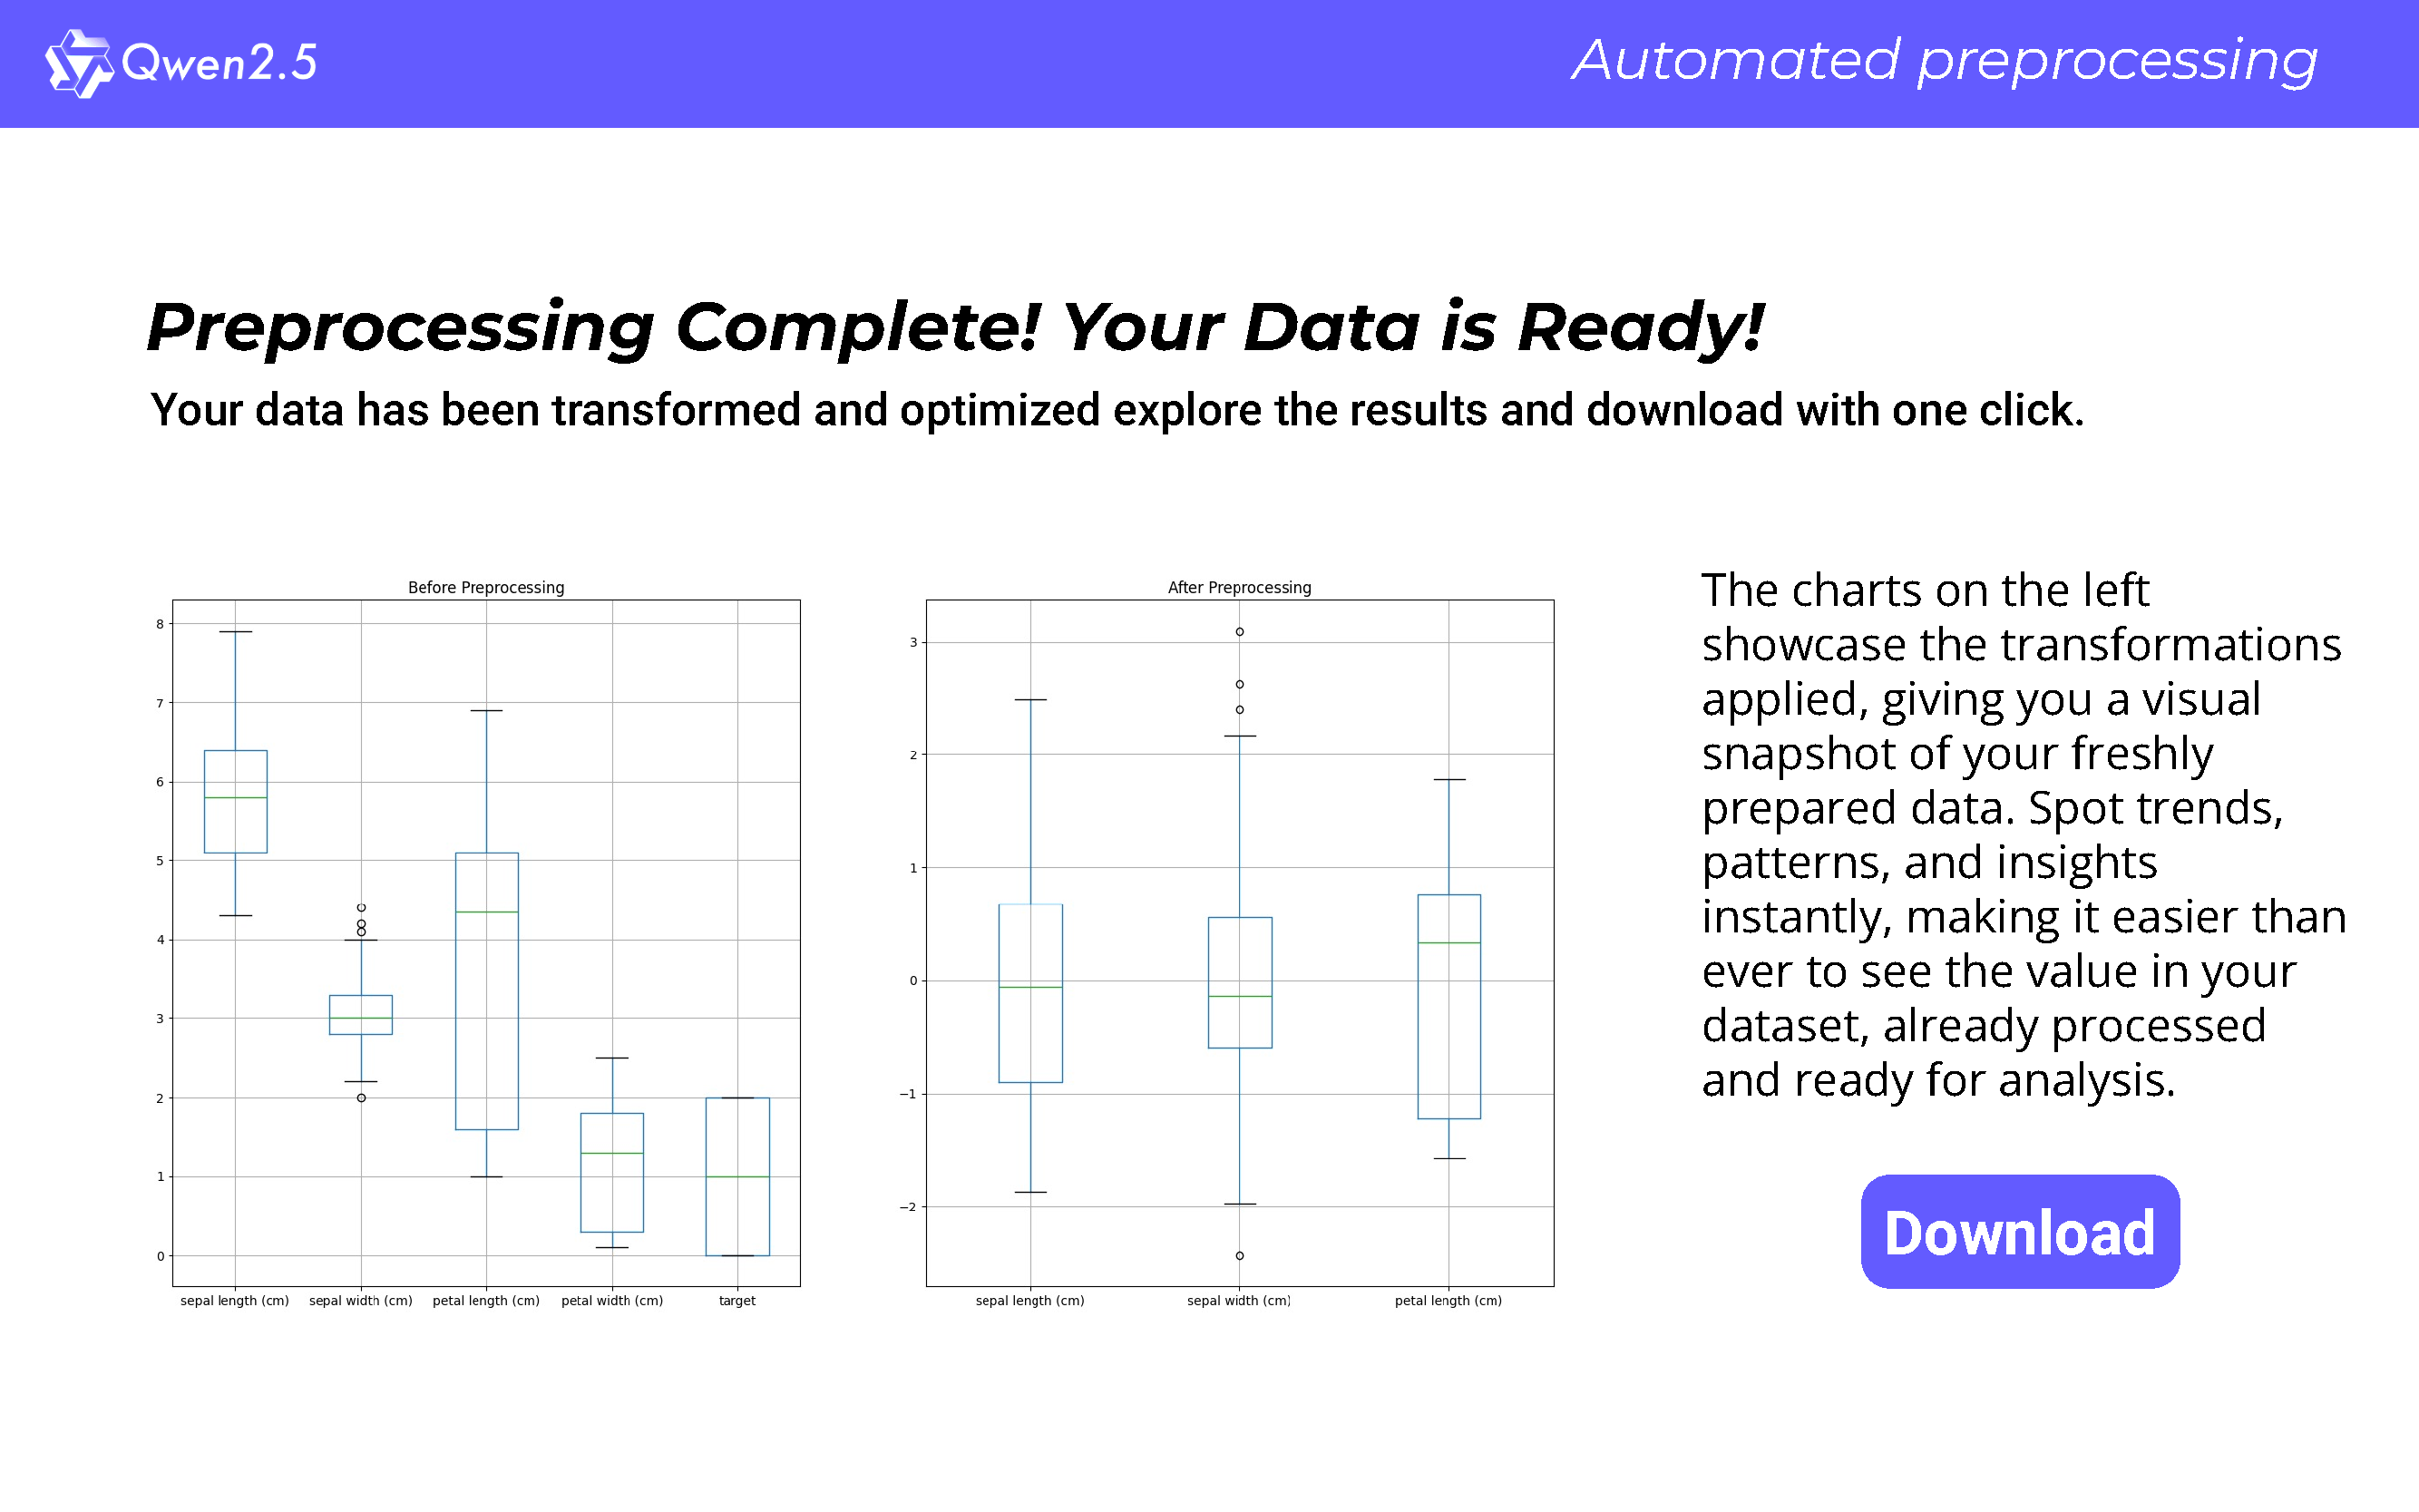
\includegraphics[width=1\textwidth]{media/App_prototipo_2.pdf}
    \caption{Results Page}\label{fig:app_mockup_2}
\end{figure}